\documentclass[../../../../document.tex]{subfiles}

\begin{document}
    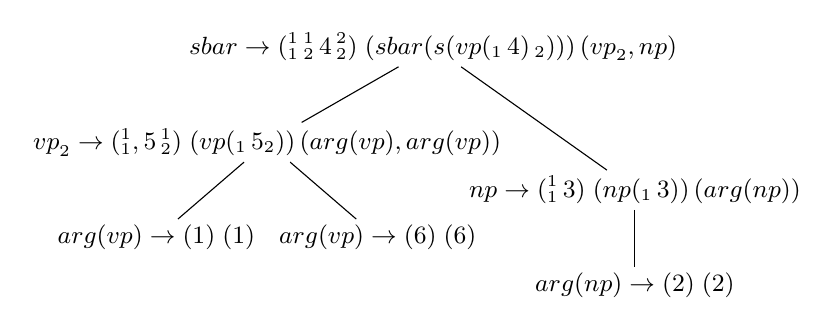
\begin{tikzpicture}[baseline=(n.north),level distance=8ex, font=\small, inner sep=2pt, level 2/.style={sibling distance=8em}, level 1/.style={sibling distance=12em}]
        \node (root) {\(\nt{sbar} \to (\x_1^1\,\x_2^1\,\tn{4}\,\x_2^2)\;(\cn{sbar} (\cn{s} (\cn{vp} (\x_1\, \tn{4})\,\x_2)))\,(\nt{vp}_2, \nt{np})\)}
        child {node (v) {\(\nt{vp}_2 \to (\x_1^1, \tn{5}\,\x_2^1)\;(\cn{vp}(\x_1 \, \tn{5} \x_2)) \,(\text{arg}(\nt{vp}), \text{arg}(\nt{vp}))\)}
            child {node {\( \text{arg}(\nt{vp}) \to (\tn{1})\;(\tn{1})\)}}
            child {node {\( \text{arg}(\nt{vp}) \to (\tn{6})\;(\tn{6})\)}}}
        child {node[yshift=-4ex, xshift=3ex] (n) {\(\nt{np} \to (\x_1^1\, \tn{3})\;(\cn{np} (\x_1 \, \tn{3}))\,(\text{arg}(\nt{np}))\)}
            child {node {\(\text{arg}(\nt{np}) \to (\tn{2})\;(\tn{2})\)}}};
    \end{tikzpicture}
\end{document}